%\documentclass[]{beamer}
%\documentclass[handout]{beamer}
\documentclass[handout,draft]{beamer}

% Preambulo
% Paquetes para usar bien el idioma español
\usepackage[spanish,es-tabla]{babel}
\selectlanguage{spanish}
\usepackage[utf8]{inputenc}

% Paquetes para usar mejores imagenes
\usepackage{graphicx}

% Paquetes para links y tabla de contenidos en el PDF
\usepackage{hyperref}
\hypersetup{colorlinks=true,allcolors=blue}
%\usepackage{hypcap}

% Paquetes para mejores tablas
\usepackage{booktabs}

% Mejor matematica
\usepackage{amsmath}

% Fuentes de las imagenes
\usepackage[absolute,overlay]{textpos}

% Paquete captions
\usepackage[justification=centering,labelformat=empty,labelsep=none]{caption}

% Opciones para ticks
\usepackage{tikz}
\usetikzlibrary{shapes,arrows,positioning}

\tikzstyle{decision} = [diamond, draw, fill=blue!20, text width=4em, text badly centered, node distance=2cm, inner sep=0pt,on grid]
\tikzstyle{block} = [rectangle, draw, fill=blue!20, text width=8em, text centered, rounded corners, minimum height=2em,on grid]
\tikzstyle{line} = [draw, -latex]

% Citas bibliograficas
\usepackage[backend=biber]{biblatex}
\renewcommand{\footnotesize}{\tiny}
\addbibresource{biblio.bib}

% Mejoro las captions
\setbeamertemplate{caption}{\raggedright\insertcaption\par}

\setbeamertemplate{caption}{%
\begin{beamercolorbox}[wd=0.85\paperwidth, sep=.2ex]{block body}\insertcaption%
\end{beamercolorbox}%
}


% Sacar barra de navegacion
\setbeamertemplate{navigation symbols}{}%remove navigation symbols

% Transparencias en items
\setbeamercovered{transparent}

% Estilo de diapositivas
% \usetheme{Boadilla}
\usecolortheme{whale}
\usecolortheme{orchid}


\title{Herramientas de Teledetección Cuantitativa\\{\small Clase 2}}
\author{Francisco Nemi\~na}
\institute[Inst.]{
\includegraphics[height=1cm]{imagenes/logosopi.png}\phantom{pepe} 
\includegraphics[height=1cm]{imagenes/2mp.png}\phantom{pepe} 
\includegraphics[height=1cm]{imagenes/conae.png}}
\date{}
%\titlegraphic{
%\includegraphics[height=1cm]{IMAGENES/minplan.png}\phantom{1}
%
\includegraphics[height=1cm]{IMAGENES/conae.png}\phantom{1}
%
\includegraphics[height=1cm]{IMAGENES/sopi.png}}

\logo{
\includegraphics[height=0.7cm]{imagenes/sopi.png}}

\AtBeginSection[]
{
\begin{frame}
\frametitle{Esquema de presentaci\'on}
\tableofcontents[currentsection]
\end{frame}
}


\begin{document}
\begin{frame}
    \maketitle
\end{frame}

\section{Transferencia radiativa}

\subsection{Planteo del problema}

\begin{frame}{Planteo del problema}
  \begin{block}{Problema}
    Queremos estudiar el problema de adquirir una imagen satelital cuando hay atm\'osfera presente.\pause
    Para esto estudiaremos la variac\'on de la radiancia.
    $$L_\lambda$$
  \end{block}
\end{frame}
%--- Next Frame ---%

\begin{frame}{Planteo del problema}
  \begin{figure}
  \centering
  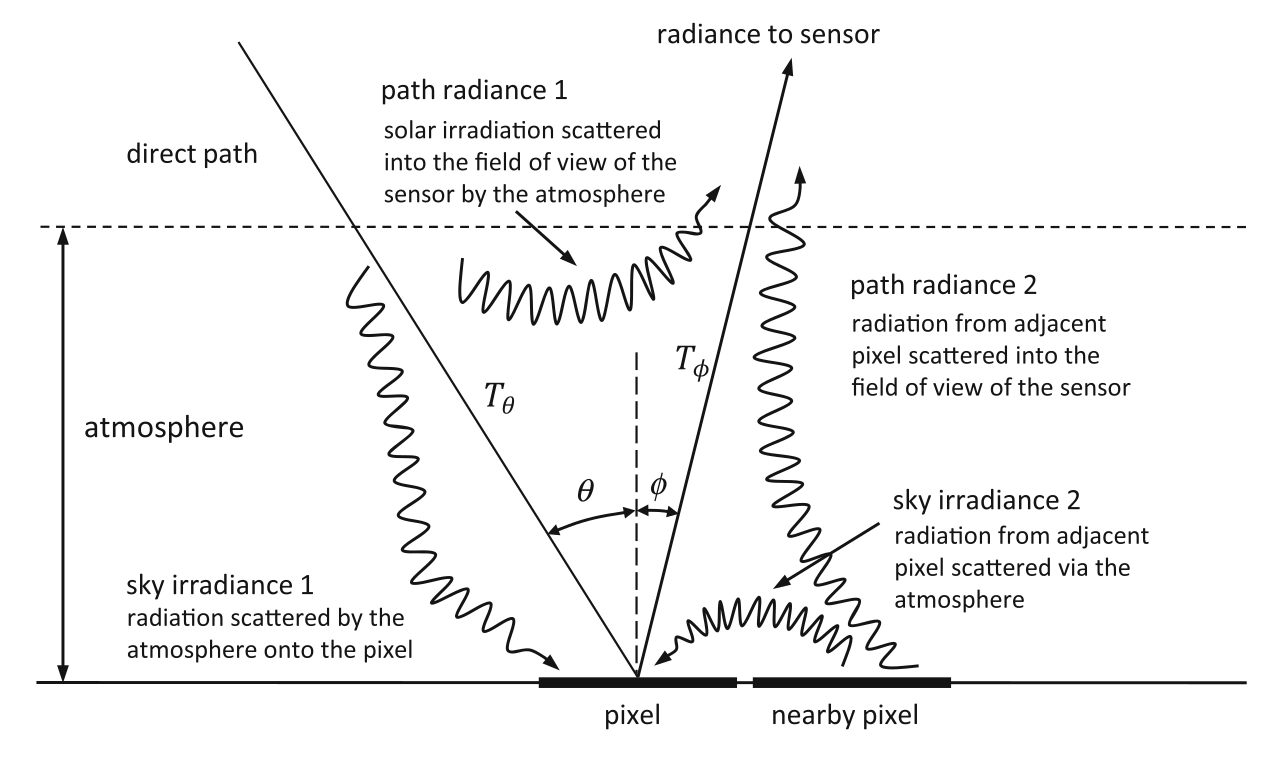
\includegraphics[width=0.8\textwidth]{imagenes/iatmo.png}
  \caption{Interacciones entre la atm\'osfera y la luz.\footfullcite{richards2013remote}}
  \end{figure}
\end{frame}
%--- Next Frame ---%

\begin{frame}{Planteo del problema}
  \begin{figure}
  \centering
  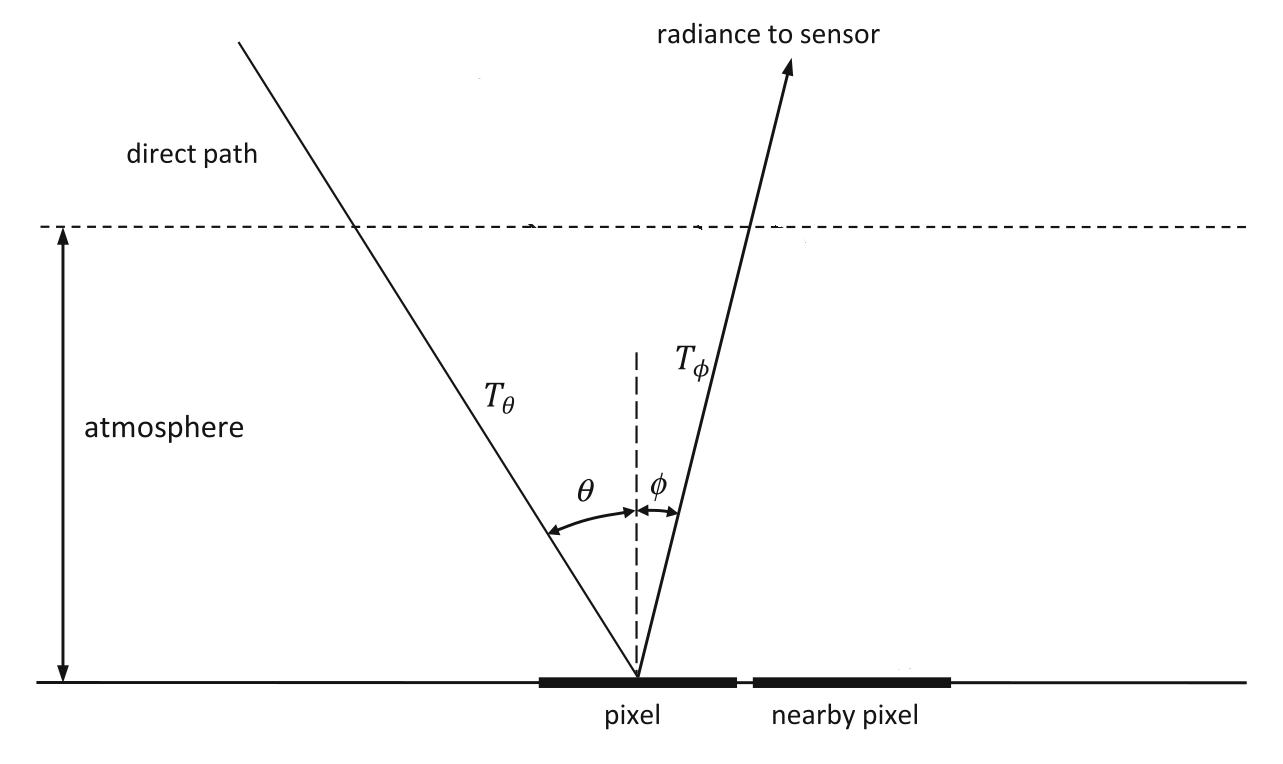
\includegraphics[width=0.8\textwidth]{imagenes/tatmo.png}
  \caption{Diagrama esquem\'atico de la absorci\'on en la atm\'osfera.\footfullcite{richards2013remote}}
  \end{figure}
\end{frame}
%--- Next Frame ---%

\begin{frame}{Planteo del problema}
  \begin{figure}
  \centering
  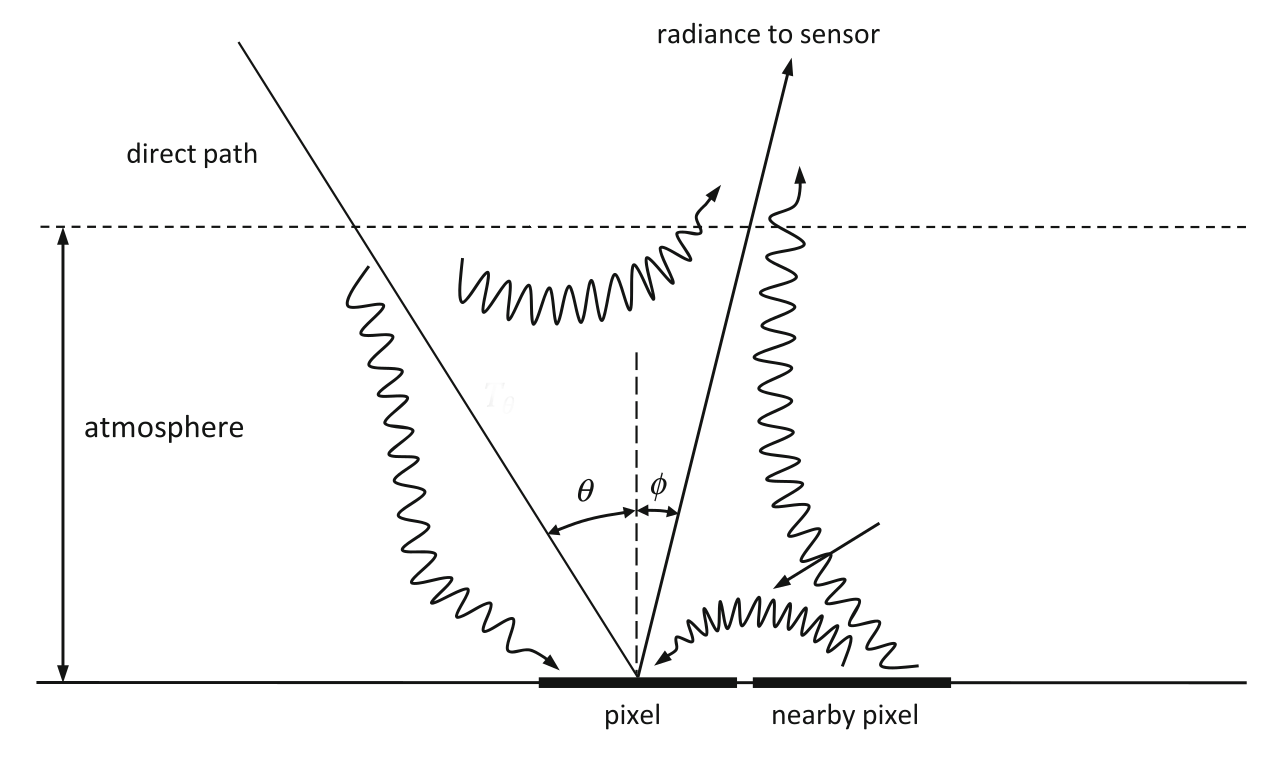
\includegraphics[width=0.8\textwidth]{imagenes/patmo.png}
  \caption{Diagrama esquem\'atico de las dispersi\'ones en la atm\'osfera.\footfullcite{richards2013remote}}
  \end{figure}
\end{frame}
%--- Next Frame ---%

\begin{frame}{Planteo del problema}
  \begin{block}{Formulaci\'on matem\'atica}
    $$d L_\lambda = -k_\lambda \rho L_\lambda ds + j_\lambda \rho ds$$
    donde $-k_\lambda \rho L_\lambda ds$ representa absorciones y $j_\lambda \rho ds$ representa fuentes, \pause
    $$ \frac{dL_\lambda}{k_\lambda \rho ds} = -L_\lambda + J_\lambda$$
  \end{block}
  \pause
  \begin{block}{Nombres}
    \begin{itemize}
      \item $k_\lambda$ mass extintion cross section
      \item $j_\lambda$ source function coefficient
      \item $\rho$ densidad
    \end{itemize}
  \end{block}
\end{frame}
%--- Next Frame ---%

\begin{frame}{Planteo del problema}
  \begin{alertblock}{Aproximaciones}
    Resolver esto en general es imposible. Tendremos que hacer distintas aproximaciones.
  \end{alertblock}
\end{frame}
%--- Next Frame ---%

\section{Aproximaciones}

\subsection{Absorci\'on constante y sin fuentes}

\begin{frame}{Absorci\'on constante y sin fuentes}
  \begin{exampleblock}{$k_\lambda = cte$, $j_\lambda = 0$}
    En este caso nos queda la ecuaci\'on
    $$ dL_\lambda = -k_\lambda \rho L_\lambda ds$$
    \pause cuya soluci\'on es
    $$ L_\lambda(s_1) = L_\lambda(0) \exp\left( -\int_0^{s_1} k_\lambda \rho ds \right)$$
  \end{exampleblock}
\end{frame}
%--- Next Frame ---%

\begin{frame}{Absorci\'on constante y sin fuentes}
  \begin{exampleblock}{$k_\lambda = cte$, $j_\lambda = 0$}
    Notando $$u = \int_0^{s_1} \rho ds$$ nos queda la ecuaci\'on mas compacta
    $$ L_\lambda(s_1) = L_\lambda(0) e^{-k_\lambda u}$$
    conocida como ley de Beer-Bouguer-Lambert.
  \end{exampleblock}
\end{frame}
%--- Next Frame ---%

\begin{frame}{Absorci\'on constante y sin fuentes}
  \begin{block}{Definici\'on}
    Llamamos transmitancia espectral al valor $$T_\lambda = \frac{L_\lambda}{L_\lambda(0)} = e^{-k_\lambda u}$$
  \end{block}\pause
  \begin{exampleblock}{Utilidad}
    Si definimos la transmitancia como arriba:
    $$L_\lambda = T_\lambda  L_\lambda(0)$$
  \end{exampleblock}
\end{frame}
%--- Next Frame ---%

\subsection{Atm\'osfera plana}

\begin{frame}{Atm\'osfera plana}
  \begin{exampleblock}{Atm\'osfera plana}
    Suponemos que toda la dependencia espacial es en la direcci\'on z, entonces $$\mu \frac{dL_\lambda}{k_\lambda \rho dz} = -L_\lambda + J_\lambda$$\pause
    definiendo a la profundidad \'optica como $$\tau_\lambda = \int_z^\infty k_\lambda \rho dz$$
  \end{exampleblock}
\end{frame}
%--- Next Frame ---%

\begin{frame}{Atm\'osfera plana}
  \begin{exampleblock}{Atm\'osfera plana}
    Nos queda entonces
    $$\mu \frac{dL_\lambda}{d\tau} = L_\lambda - J_\lambda$$\pause
    resolver esto ya depende de la atm\'osfera y no suele haber formas cerradas.
  \end{exampleblock}
  \pause
  \begin{alertblock}{Observacion}
    Necesito adem\'as conocer 2 condiciones de contorno.
    \begin{itemize}
      \item La radiancia solar
      \item La reflectancia en el terreno
    \end{itemize}
  \end{alertblock}
\end{frame}
%--- Next Frame ---%

\section{Atm\'osfera}

\begin{frame}{atm\'osfera}
  \begin{block}{Efectos atmosfericos}
    \begin{itemize}
      \item<1-3> Absorciones
      \begin{itemize}
        \item<2-3> Constantes
        \item<3> Variables
      \end{itemize}
      \item<4-7> Dispersi\'on
      \begin{itemize}
        \item<5-7> Rayleigh
        \item<6-7> Mie
        \item<7> Aerosoles
      \end{itemize}
    \end{itemize}
  \end{block}
\end{frame}
%--- Next Frame ---%

\subsection{Absorciones}

\begin{frame}{Absorciones}
  \begin{figure}
  \centering
  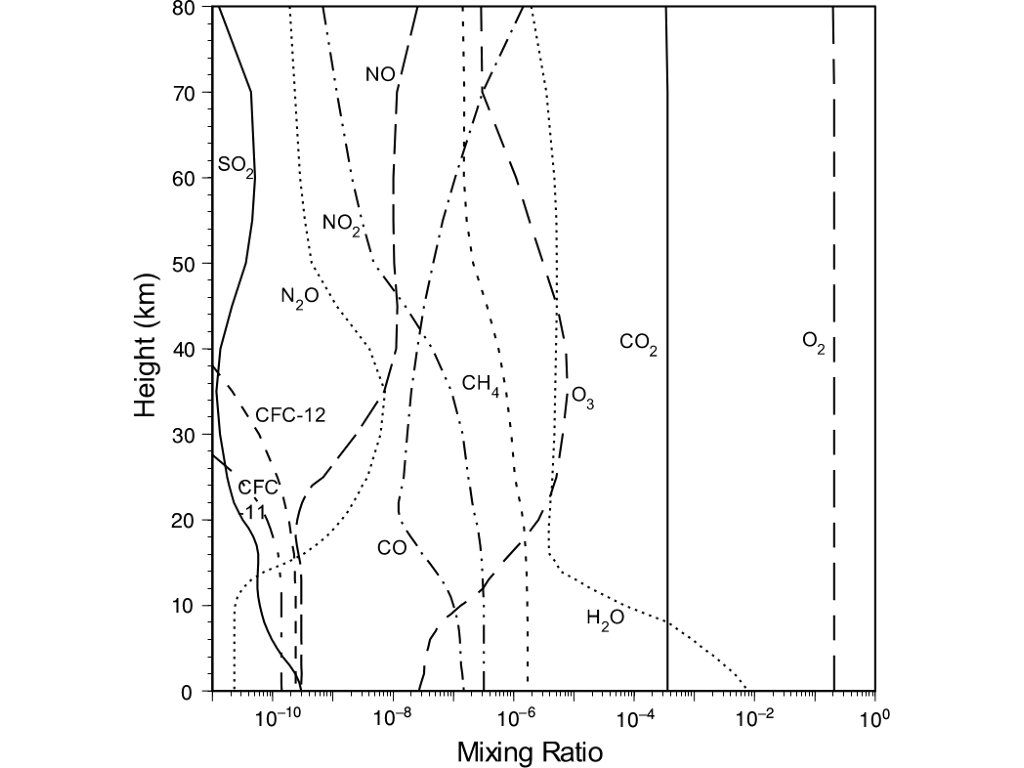
\includegraphics[width=0.8\textwidth]{imagenes/composicion.png}
  \caption{Composici\'on de la atm\'osfera.\footfullcite{liou2002introduction}}
  \end{figure}
\end{frame}
%--- Next Frame ---%

\begin{frame}{Absorciones}
  \begin{figure}
  \centering
  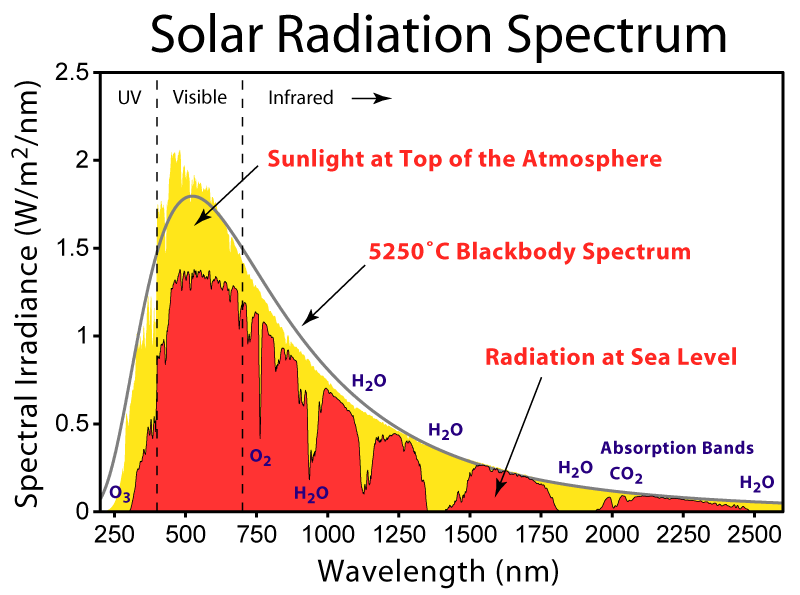
\includegraphics[width=0.7\textwidth]{imagenes/solar_spectrum.png}
    \caption{Comparaci\'on entre la irradiancia solar a tope de la atm\'osfera y de la cobertura.\footfullcite{solar_spectrum}}
  \end{figure}
\end{frame}
%--- Next Frame ---%

\begin{frame}{Absorciones}
  \begin{figure}
  \centering
  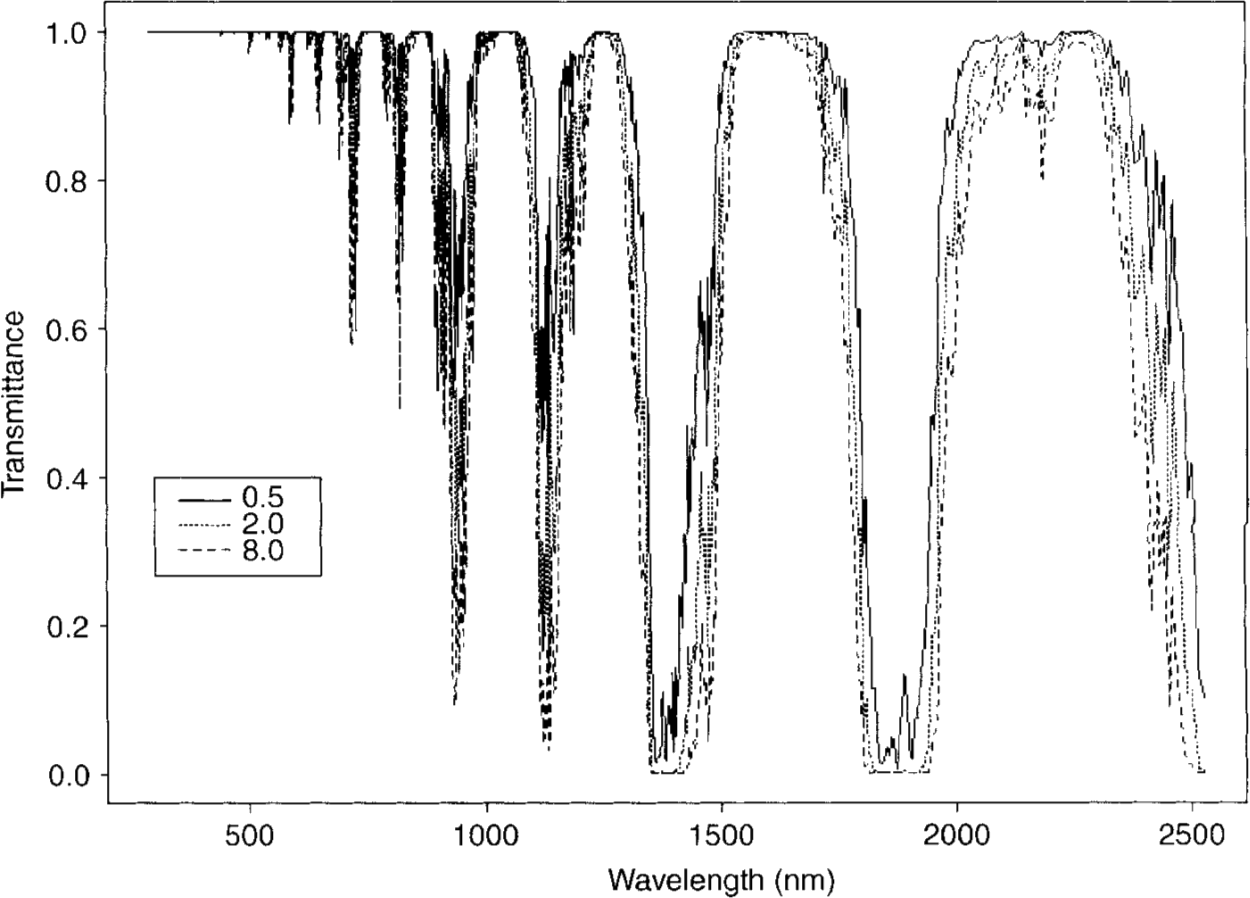
\includegraphics[width=0.8\textwidth]{imagenes/vapor.png}
  \caption{Variaciones de la absorci\'on por contenido de vapor de agua.\footfullcite{liang2005quantitative}}
  \end{figure}
\end{frame}
%--- Next Frame ---%


\begin{frame}{Absorciones}
  \begin{exampleblock}{Porcentaje de absorcion tipica}
    Para Landat 5 - TM
    \begin{figure}
      \begin{tabular}{l c c}
        Banda & Ozono  & Vapor de agua    \\
        $490\pm60 nm$& $\searrow$ 1.5\% - 2.9\%     & -  \\
        $575\pm75 nm$& $\searrow$ 5.2\% - 13.4\%    & $\searrow$ 0.5\%-3\%  \\
        $670\pm70 nm$& $\searrow$ 3.1\% - 7.9\%     & $\searrow$ 0.5\%-3\%  \\
        $837\pm107 nm$& -                 & $\searrow$ 3.5\%-14\%  \\
        $1692\pm178 nm$& -                 & $\searrow$ 5\%-16\% \\
        $2190\pm215 nm$& -                 & $\searrow$ 2.5\%-13\% \\
      \end{tabular}
      \caption{Variaciones de absorvancia por contenidod de ozono y vapor de agua. \footfullcite{vermote49atmospheric}}
    \end{figure}
  \end{exampleblock}
\end{frame}
%--- Next Frame ---%

\begin{frame}{Absorciones}
  \begin{figure}
  \centering
  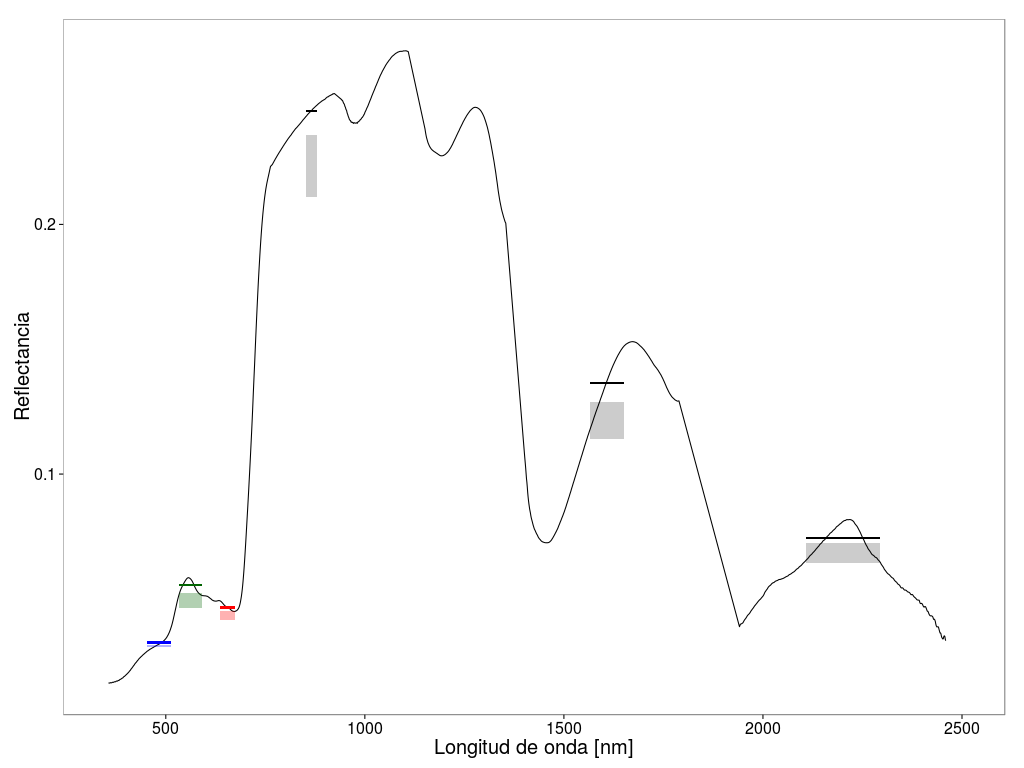
\includegraphics[width=0.7\textwidth]{imagenes/abs_veg_esp.png}
  \caption{Comparaci\'on entre la firma espectral y la respuesta espectral para vegetaci\'on con errores por absorci\'on de ozono y vapor de agua.\footfullcite{clark2007usgs}}
  \end{figure}
\end{frame}
%--- Next Frame ---%


\begin{frame}{Absorciones}
  \begin{block}{Soluciones}
   \begin{itemize}
     \item<1-> Resolver la ecuaci\'on de transferencia radiativa.
     \item<2>  Calibrar con datos en el terreno.
   \end{itemize}
  \end{block}
\end{frame}
%--- Next Frame ---%

\subsection{Dispersi\'on}

\begin{frame}{Dispersi\'on}
  \begin{figure}
  \centering
  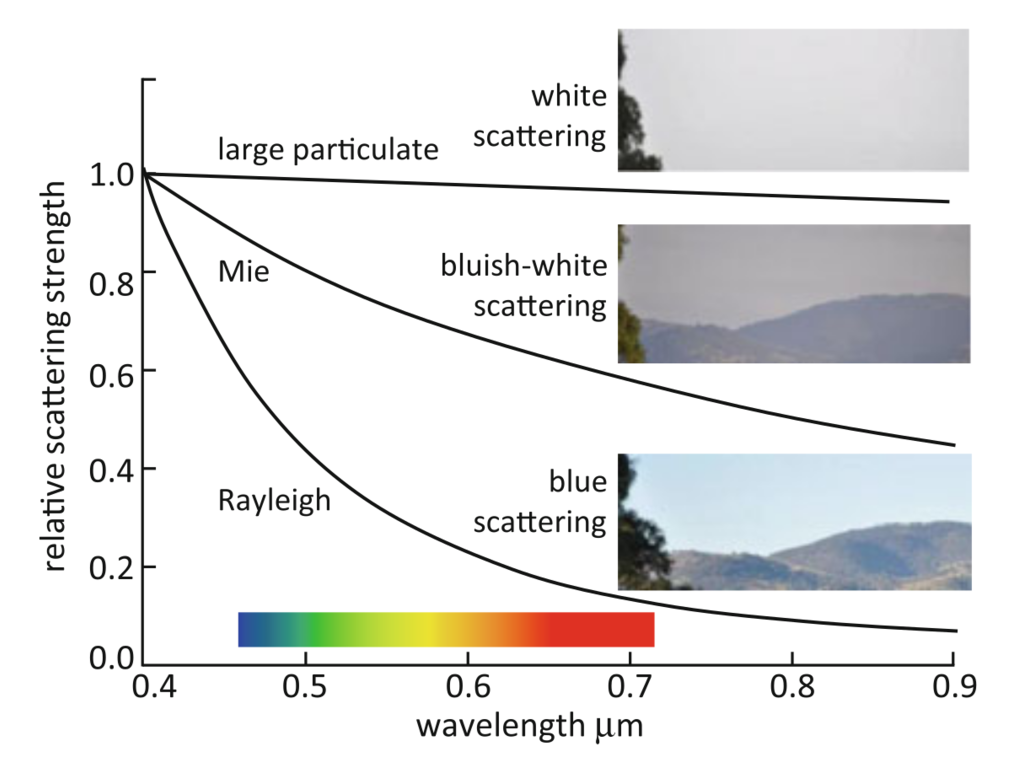
\includegraphics[width=0.8\textwidth]{imagenes/dispersion.png}
  \caption{Distintos tipos de dispersi\'on en la atm\'osfera.\footfullcite{richards2013remote}}
  \end{figure}
\end{frame}
%--- Next Frame ---%

\begin{frame}{Dispersi\'on}
  \begin{block}{Dispersi\'on de Rayleigh}
    Se da por particulas pequeñas
    $$ d << \lambda$$
    \pause esta siempre presente
    $$J_\lambda \sim \frac{1}{\lambda^4}$$
  \end{block}
\end{frame}
%--- Next Frame ---%

\begin{frame}{Dispersi\'on}
  \begin{figure}
  \centering
  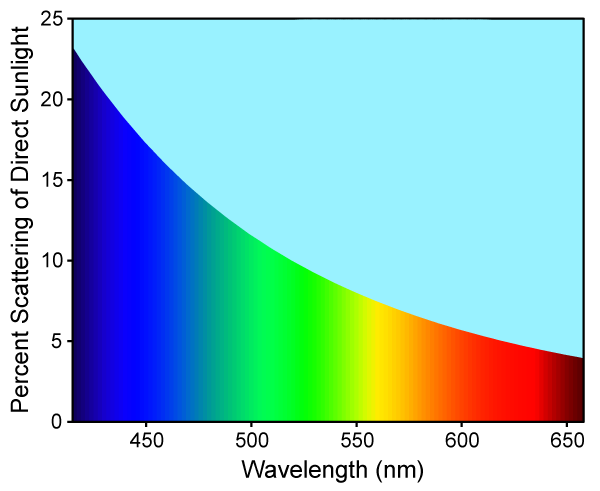
\includegraphics[width=0.6\textwidth]{imagenes/rayleigh_sunlight_scattering.png}
  \caption{$J$ vs. $\lambda$ en la zona \'optica.\footfullcite{rayleigh_sunlight_scattering}}
  \end{figure}
\end{frame}
%--- Next Frame ---%

\begin{frame}{Dispersi\'on}
  \begin{figure}
  \centering
  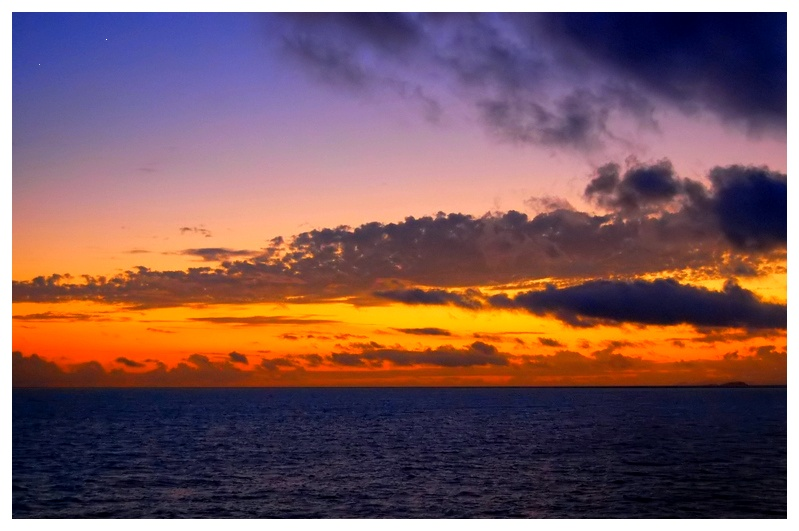
\includegraphics[width=0.8\textwidth]{imagenes/sunset.png}
  \caption{Foto de un atardecer para distender.\footfullcite{sunset}}
  \end{figure}
\end{frame}
%--- Next Frame ---%

\begin{frame}{Dispersi\'on}
  \begin{block}{Dispersi\'on de Mie}
    Se da por particulas de tamaño similar a la longitud de onda
    $$ d \sim \lambda$$
    \pause puede o no estar presente.
  \end{block}
\end{frame}
%--- Next Frame ---%

\begin{frame}{Dispersi\'on}
  \begin{block}{Dispersi\'on por aerosoles}
    Se da por particulas de mayor que la longitud de onda
    $$ d >> \lambda$$
    \pause puede estar presente en distintas zonas de la imagen.
  \end{block}
\end{frame}
%--- Next Frame ---%


\begin{frame}{Absorciones}
  \begin{exampleblock}{Porcentaje de dispersi\'on tipica}
    Para Landat 5 - TM
    \begin{figure}
      \begin{tabular}{l c c}
        Banda & Rayleigh  & Aerosol    \\
        $490\pm60 nm$& $\nearrow$ 0.064 - 0.080   & $\nearrow$ 0.007 - 0.048 \\
        $575\pm75 nm$& $\nearrow$ 0.032 - 0.040   & $\nearrow$ 0.006 - 0.040  \\
        $670\pm70 nm$& $\nearrow$ 0.018 - 0.020   & $\nearrow$ 0.005 - 0.034 \\
        $837\pm107 nm$& $\nearrow$ 0.007 - 0.009  & $\nearrow$ 0.003 - 0.023 \\
        $1692\pm178 nm$& $\nearrow$ 0.000 - 0.001  & $\nearrow$ 0.001 - 0.007 \\
        $2190\pm215 nm$& -                         & $\nearrow$ 0.001 - 0.004 \\
      \end{tabular}
    \end{figure}
  \end{exampleblock}
\end{frame}
%--- Next Frame ---%

\begin{frame}{Dispersi\'on}
  \begin{figure}
  \centering
  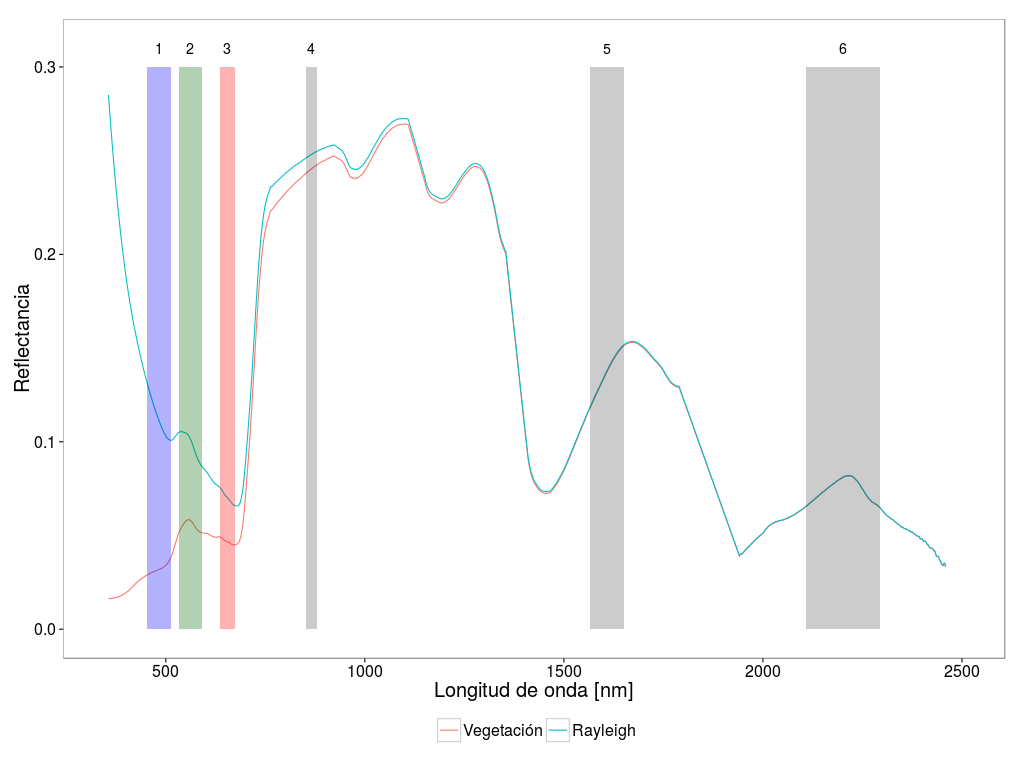
\includegraphics[width=0.8\textwidth]{imagenes/rayleigh.png}
  \caption{Variacion de la firma espectral por dispersi\'on de Rayleigh. \footfullcite{clark2007usgs}}
  \end{figure}
\end{frame}
%--- Next Frame ---%

\begin{frame}{Dispersi\'on}
  \begin{block}{Soluciones}
   \begin{itemize}
     \item<1-> Resolver ecuaci\'on de transferencia radiativa
     \item<2-> Calibrar con datos en el terreno.
     \item<3>  Modelar al comportamiento de forma estadistica.
   \end{itemize}
  \end{block}
\end{frame}
%--- Next Frame ---%

\section{Soluciones practicas}

\subsection{Reflectancia}

\begin{frame}[fragile]{Reflectancia}
  \begin{block}{Calculo}
    $$ \rho_{toa} = \frac{\pi L}{E_0}$$ \pause
    \begin{center}
    \verb| 3.14 * d^2 (g * DN + b) / E0 | \pause
    \end{center}
    \begin{itemize}
      \item \verb+DN+ : n\'umero digital
      \item \verb+g+ : ganancia
      \item \verb+b+ : bias
      \item \verb+d+ : distancia tierra-sol
      \item \verb+E_0+ : irradiancia solar
    \end{itemize}
  \end{block}
\end{frame}
%--- Next Frame ---%

\begin{frame}[fragile]{Angulo solar}
  \begin{block}{Calculo}
    $$ \rho_{\cos} = \frac{\rho_{toa}}{\cos(\theta)}$$ \pause
    \begin{center}
    \verb| DN / cos(a)  | \pause
    \end{center}
    \begin{itemize}
      \item \verb+DN+ : reflectancia
      \item \verb+a+ : \'angulo solar
    \end{itemize}
  \end{block}
\end{frame}
%--- Next Frame ---%

\subsection{Correccion atmosferica}

\begin{frame}[fragile]{DOS1}
  \begin{block}{Calculo}
    $$ \rho_{dos} = \frac{\rho_{toa} - \rho_p}{\cos(\theta)}$$ \pause
    \begin{center}
    \verb| (DN - DNmin) / cos(a)  | \pause
    \end{center}
    \begin{itemize}
      \item \verb+DN+ : reflectancia
      \item \verb+DNmin+ : reflectancia m\'inima de la banda
      \item \verb+a+ : \'angulo solar
    \end{itemize}
  \end{block}
\end{frame}
%--- Next Frame ---%

\begin{frame}{DOS1}
  \begin{figure}
  \centering
  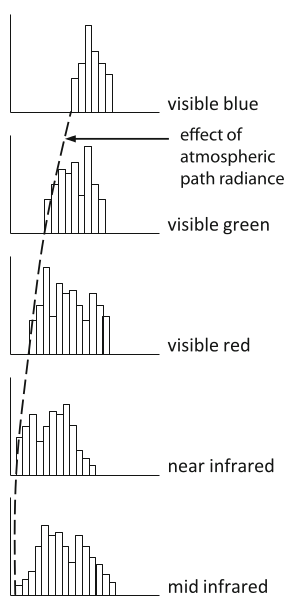
\includegraphics[width=0.30\textwidth]{imagenes/dos.png}
  \caption{Histogramas por banda mostrando el menor valor en cada una.\footfullcite{richards2013remote}}
  \end{figure}
\end{frame}
%--- Next Frame ---%

\begin{frame}[fragile]{Objetos pseudoinvariantes}
  \begin{block}{Calculo}
    $$ \rho_{pse} = A * \rho_{toa} + B$$ \pause
    donde $A$ y $B$ se obtienen a partir de encontrar objetos invariantes en cada imagen.
  \end{block}
\end{frame}
%--- Next Frame ---%

\section{Pr\'actica}

\begin{frame}{Pr\'actica}
  \begin{exampleblock}{Actividades pr\'acticas de la segunda clase}
    \begin{enumerate}
      \item Abrir im\'agenes Landsat 8 y digitalizar coberturas de interes.
      \item Convertir la imagen a reflectancia.
      \item Corregir la imagen por el coseno del angulo.
      \item Corregir la imagen por DOS 1\%.
      \item Corregir la imagen por objetos invariantes
      \item Comparar las firmas obtenidas por distintos metodos.
    \end{enumerate}
  \end{exampleblock}
\end{frame}
%--- Next Frame ---%


\end{document}
